\documentclass[12pt,letterpaper]{article}
\usepackage{fullpage, lastpage, enumerate, fancyhdr, titlesec}
\usepackage[top=2cm, bottom=4.5cm, left=2.5cm, right=2.5cm]{geometry}
\usepackage{amsmath,amsthm,amsfonts,amssymb,amscd}
\usepackage{mathrsfs, xcolor, graphicx, subcaption, siunitx}
\usepackage{hyperref}
\graphicspath{{./images}}

\hypersetup{%
  colorlinks=true,
  linkcolor=blue,
  linkbordercolor={0 0 1}
}

\setlength{\parindent}{0.0in}
\setlength{\parskip}{0.05in}

\titleformat{\subsection}
  {\normalfont\normalsize\itshape}{\thesubsection}{1em}{}

\pagestyle{fancyplain}
\headheight 15pt
\fancyhf[FL]{Matthew Bernstein}
\fancyhf[HR]{\today}
\fancyhf[HL]{ISyE 7406 - Homework 4}
\fancyhf[FC]{}
\fancyhf[FR]{\thepage}
\headsep 1.5em

\title{ISYE 7406 - Homework 4}
\author{Matthew Bernstein}

\begin{document}
\fancypagestyle{plain}{
    \fancyhf{}
    \renewcommand{\headrulewidth}{0pt}
    \renewcommand{\footrulewidth}{0pt}
}
\maketitle

\section*{Introduction}
\section*{Exploratory Data Analysis}
\section*{Methodology}

In order to test the various local smoothing methods, two sets of points that fit the "mexican hat function":
\begin{equation}
    f(x) = (1-x^2)exp(-0.5 x^2)\;\; -2\pi \le x \le 2\pi
\end{equation}
One of the set of points is equidistant in the range $[-2\pi, 2\pi]$. The other set is deterministic. 

For each set of points, Gaussian jitter of form $\mathcal{N}(0,0.2^2)$ is added to each point and then 3 separate local smoothing methods are applied to the new data points:
\begin{enumerate}
    \item LOESS
    \item Nadaraya-Watson Kernel Smoothing with a Gaussian Kernel
    \item Splines Smoothing
\end{enumerate}

1000 trials for each sets points which the Gaussian jitter regenerated each time. The results at each $x_i$ are aggregated and bias, variance, and MSR are calculated.

\section*{Results}

\subsection*{Equidistant Point Set}

\begin{figure}[!htp]
    \caption{Results from Part 1, equidistant point set}
    \centering
    \begin{subfigure}{0.45\textwidth}
      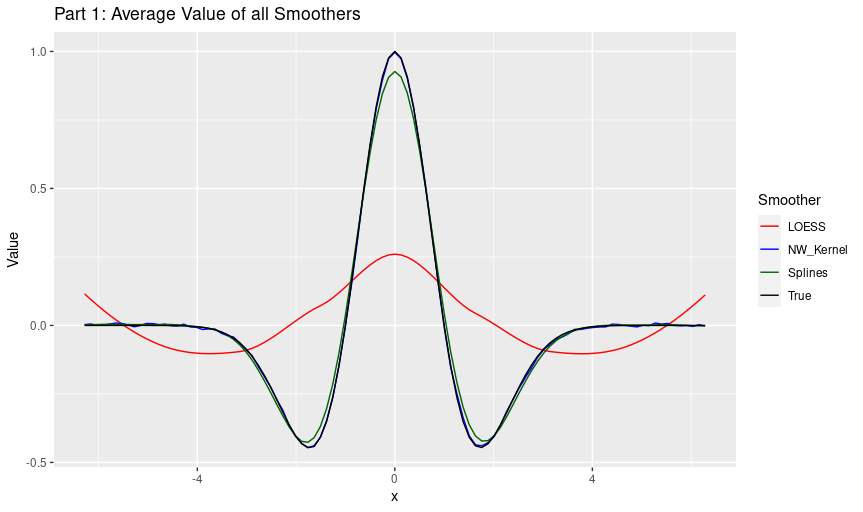
\includegraphics[width=\textwidth]{p1_value}
    \end{subfigure}
    \begin{subfigure}{0.45\textwidth}
      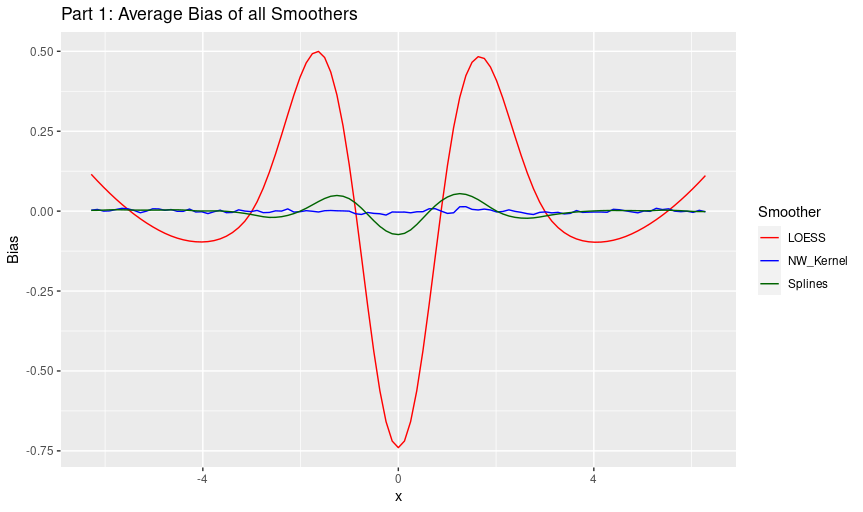
\includegraphics[width=\textwidth]{p1_bias}
    \end{subfigure}
    \begin{subfigure}{0.45\textwidth}
      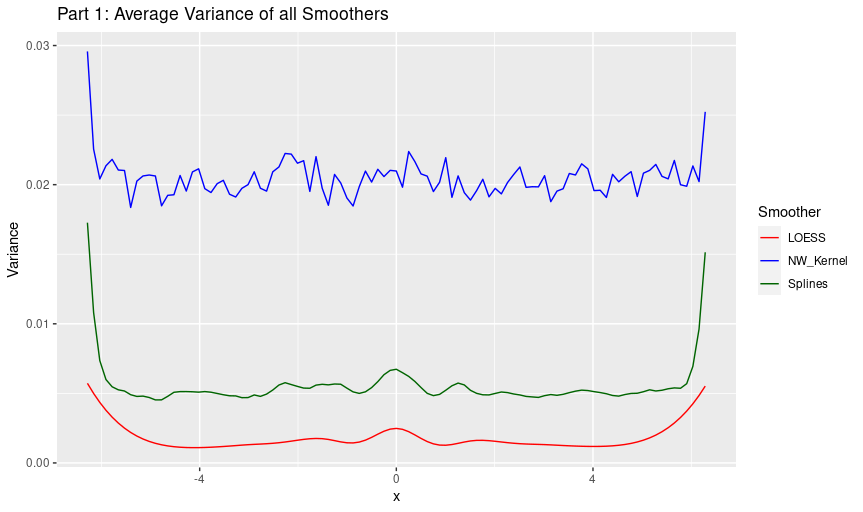
\includegraphics[width=\textwidth]{p1_var}
    \end{subfigure}
    \begin{subfigure}{0.45\textwidth}
        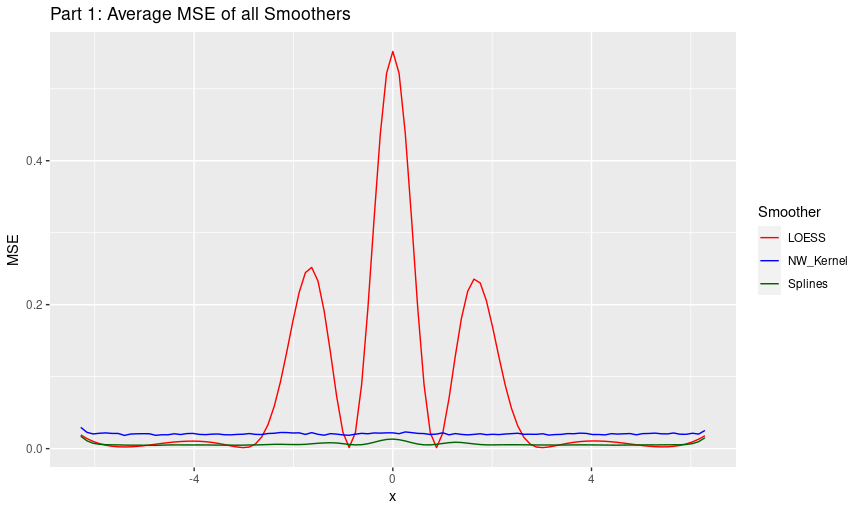
\includegraphics[width=\textwidth]{p1_mse}
      \end{subfigure}
    \label{fig:part1}
\end{figure}

Figure \ref{fig:part1} shows the results from the equidistant point set. Kernel and Splines smoothing appear to fit the true data set very closely. Both have extremely low bias and MSE throuhgout the domain, although kernel smoothing has siginificantly more variance. LOESS was the most consistent smoothing methods but also the least accurate, this is could be due to an extremely high span parameter of 0.75 meaning of the 101 total points used, around 75 of them are used in the local smoothing and so points from far away affect the models smoothing. Interestingly, all smoothing algorithms have higher variance at the tails of the domain. 

\subsection*{Deterministic Point Set}

\begin{figure}[!htp]
    \caption{Results from Part 2, deterministic point set}
    \centering
    \begin{subfigure}{0.45\textwidth}
      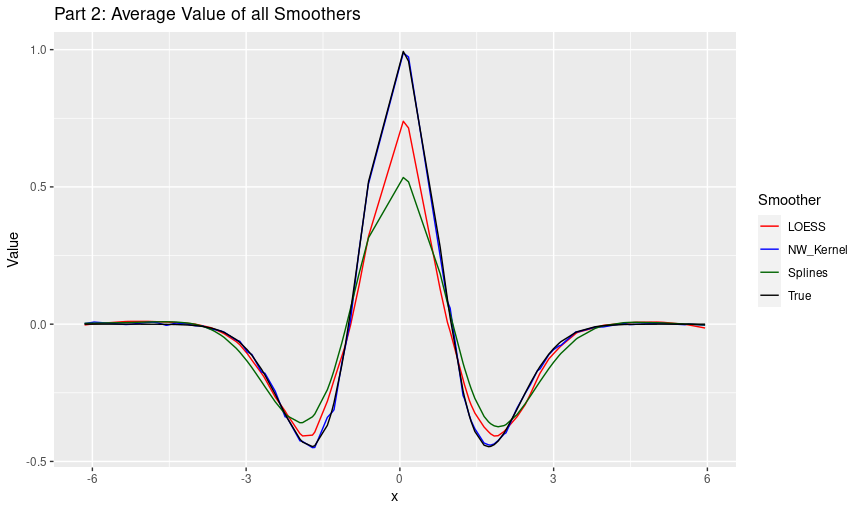
\includegraphics[width=\textwidth]{p2_value}
    \end{subfigure}
    \begin{subfigure}{0.45\textwidth}
      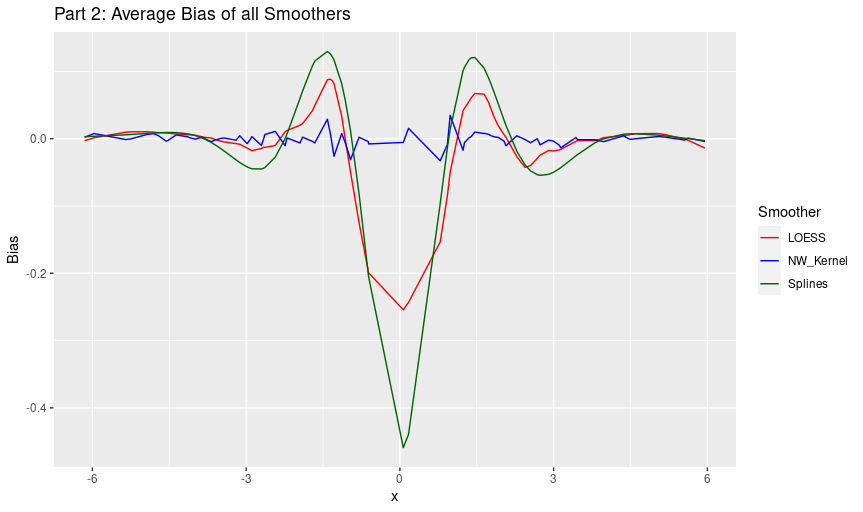
\includegraphics[width=\textwidth]{p2_bias}
    \end{subfigure}
    \begin{subfigure}{0.45\textwidth}
      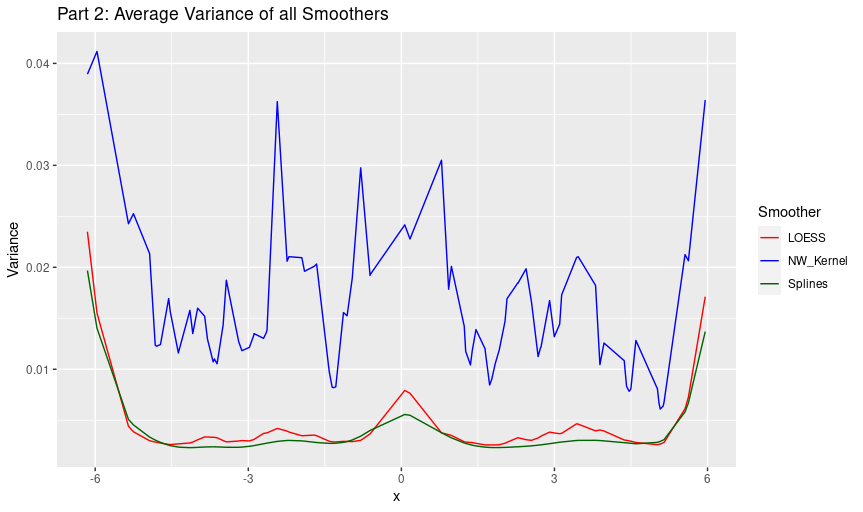
\includegraphics[width=\textwidth]{p2_var}
    \end{subfigure}
    \begin{subfigure}{0.45\textwidth}
        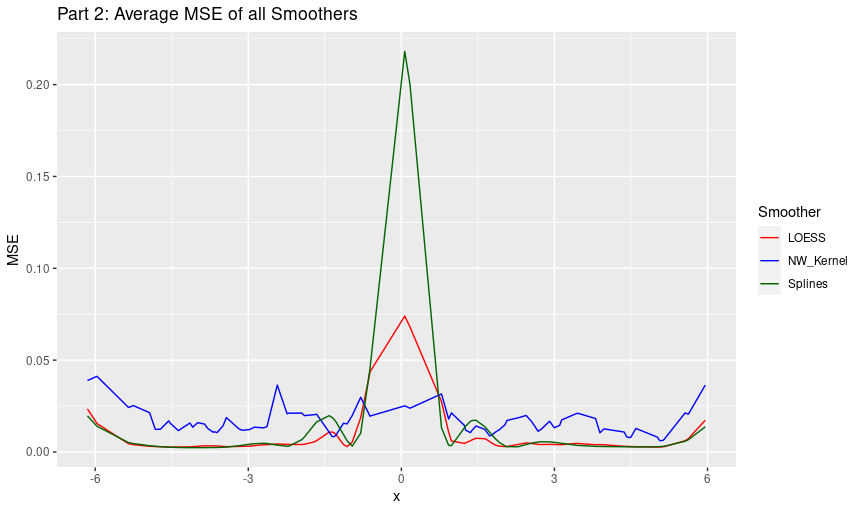
\includegraphics[width=\textwidth]{p2_mse}
      \end{subfigure}
    \label{fig:part2}
\end{figure}

Figure \ref{fig:part2} shows the results of the deterministic point set. All three smoothing methods are fairly similar in this point set. Kernel smoothing is again the most accurate but also has the highest variance. Splines smoothing is the least accurate of the three in this point set, this is somewhat to be expected since spline smoothing relies on equidistant points. The lower $\alpha$ value in the LOESS smoothing contributes to a more accurate model as well. 

\section*{Conclusion}

Each of the three smoothing algorithms can perform well in smoothing a difficult to estimate functions. Spline smoothing performs siginificantly better given an equidistant point set. LOESS smoothing can be particularly sensitive to the chosen smoothing parameter. Given the two data sets, it appeared that kernel smoothing was the most accurate, however with the highest variance so could be unreliable in lower iteration. In conclusion, each method has its strengths and weaknesses and are all valid methods for local smoothing.

\end{document}